\section{The Riemann problem}
We will now define the Riemann problem, since it plays a crucial role in the finite volume method.
In the Riemann problem we distinguish between what we call a wet bed and a dry bed. 
A wet bed is the case where the water depth is positive everywhere, whereas a dry bed is the case where the water depth is zero in some cells.
The special Riemann problem where parts of the bed are dry is dealing with the so-called dry fronts or wet/dry fronts, which are challenging to handle numerically.
We will leave these cases for now, and only consider wet bed problems.
The Riemann problem for the shallow water equations in 1D with a zero source term is defined as the initial-value problem (IVP)~\cite{Toro2024}:
\begin{equation}\label{eq:Riemann_problem}
    \begin{aligned}
        \text{PDEs: } &\mathbf{U}_t + {\mathbf{F(U)}}_x = 0, \\
        \text{ICs: } &\mathbf{U}(x, 0) = \begin{cases}
            \mathbf{U_L}, & \text{if  } x < 0, \\
            \mathbf{U_R}, & \text{if  } x > 0.
        \end{cases}
    \end{aligned}
    \end{equation}
The vectors $\mathbf{U}$ and $\mathbf{F(U)}$ in~\eqref{eq:Riemann_problem} are given by
\begin{align}
    \mathbf{U} = \begin{bmatrix}
        h \\ hu \\ hv
    \end{bmatrix}, \quad
    \mathbf{F(U)} = \begin{bmatrix}
        hu \\ hu^2 + \frac{1}{2}gh^2 \\ hvu
    \end{bmatrix},
\end{align}
and the initial conditions $\mathbf{U_L}$ and $\mathbf{U_R}$ are
\begin{align*}
    \mathbf{U_L} = \begin{bmatrix}
        h_L \\ h_L u_L \\ h_L v_L
    \end{bmatrix}, \quad 
    \mathbf{U_R} = \begin{bmatrix}
        h_R \\ h_R u_R \\ h_R v_R
    \end{bmatrix},
\end{align*}
which represents the conditions at time $t = 0$ in the left and right states of $x=0$, respectively.
The function $\mathbf{U}$ is piecewise constant, with a discontinuity at $x=0$.
The Riemann problem can be solved either exactly or approximately.
Various approximate Riemann solvers exist, based on finding an approximate solution to the Riemann problem.
Some of these solvers will be considered later in the thesis.

\subsection{The Dam-Break problem}
We now introduce the dam-break problem, a scenario of significant physical interest.
This problem models the sudden release of water following the collapse of a dam, making it highly relevant for studying natural disasters such as floods and tsunamis.
As a classic test case for numerical methods, the dam-break problem is commonly used to test the ability of a method to capture discontinuities in the solution.
The dam-break problem is a special case of the Riemann problem~\eqref{eq:Riemann_problem}.
The difference is that in the dam-break problem, the initial velocity components, $u_L, u_R, v_L$ and $v_R$, are zero, whereas in the Riemann problem they are allowed to be distinct from zero.
The initial setup is visualized in Figure~\ref{fig:dam-break-problem}.
\begin{figure}[H]
    \centering
    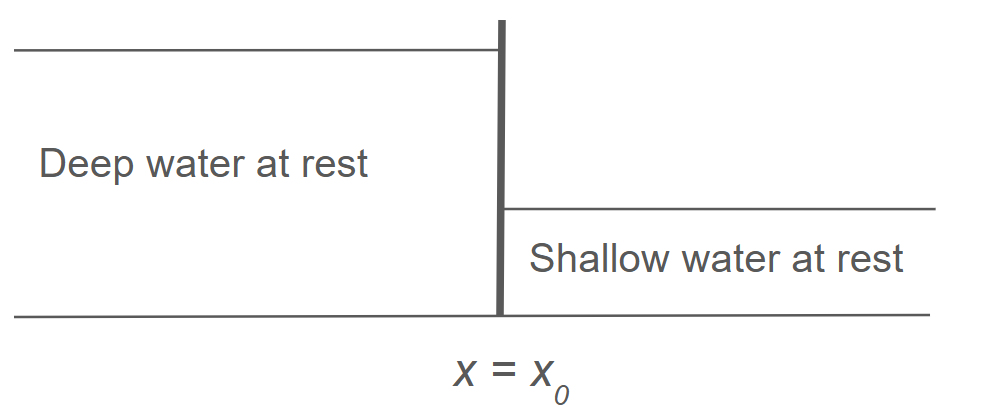
\includegraphics[width=0.5\textwidth]{C:/Users/Matteo/Shallow-Water-Equations/figs/dam-break-problem.png}
    \caption{Initial conditions for the dam-break problem. An infinitely thin wall at $x=x_0$ divides two sections of water with different water levels.}\label{fig:dam-break-problem}
\end{figure}
We can use the shallow water equations to model the flow of water in the dam-break problem, approximately, if we assume that the wall collapses instantaneously at $t=0$.

\subsection{Waves in the Riemann problem}
To get a better understanding of the flow in shallow water, we provide some very short background information about waves.
In particular the wave structure in the solution of the Riemann problem~\eqref{eq:Riemann_problem}, which consists of a combination of waves, including shock waves and rarefaction waves.
In the solution of the Riemann problem~\eqref{eq:Riemann_problem} there are four possible wave patterns outcomes, which are combinations of shock waves and rarefaction waves.
In each case there are three waves, the left and right waves correspond to the one-dimensional SWE, and the middle wave aries from the $y-$momentum equation in~\eqref{eq:Riemann_problem} and is always a shear wave.
The left and right waves are either shock waves or rarefaction waves.
The four possible wave patterns are as follows:
(a) Left rarefaction, right shock, (b) Left shock, right rarefaction, (c) Both left and right rarefaction, and (d) Both left and right shock.
In the example of the dam-break problem, with inital conditions as in Figure~\ref{fig:dam-break-problem}, the solution consists of a left rarefaction wave and a right shock wave.

%Hence the structure of the solution in general is shown in the figure below.
%From the figure we see that the solution consists of three waves, a left wave, a middle wave and a right wave, which together seperate four regions, described by the vector
%\begin{align*}
%\mathbf{W} = \begin{bmatrix}
%    h \\ hu \\ hv
%    \end{bmatrix}.
%\end{align*}
%The four regions are describes by $\mathbf{W}_L$ (left data), $\mathbf{W}_R$ (right data), $\mathbf{W}_{*L}$ and $\mathbf{W}_{*R}$, which both denote star region data.
%We are interested in the star region data, since these are the unknowns.
%Based on the given initial conditions, we must determine the types of waves.
%Second, it is known that across the left and right waves, both $h$ and $u$ change but $v$ remains constant.
%Whereas across the middle wave, $v$ changes but $h$ and $u$ remain constant.
%That is, $h$ and $u$ remain constant in the star region.
%Thus the water depth and particle velocity are constant in the star region and are denoted by $h_*$ and $u_*$, respectively.

\subsection{Exact Riemann solver}
The exact Riemann solver is a method that solves the Riemann problem exactly, and it is based on the solution of the Riemann problem~\eqref{eq:Riemann_problem}.
There exist exact Riemann solvers which are very efficient and leads to Gudonov methods, that are only slightly more expensive than those based on approximate Riemann solvers~\cite{Toro2001-Shock}.
However, in this project we will focus on approximate Riemann solvers, which are able to solve the Riemann problem with high accuracy and efficiency.

%But for now, we will consider the case where the solution consists of a single non-trivial wave and all other waves are assumed to have zero strenght.
%This is enough to solve the Riemann problem as it is always possible to solve the Riemann problem by considering one wave at a time.
%We denote the constant values of the water depth and particle velocity in the star region by $h_*$ and $u_*$, respectively.

